\chapter{绪论}
\label{chap:intro}

\section{研究背景及意义}
互联网、移动互联网和物联网快速发展,以及5G技术的不断推进和商用推广,社交网络、位置服务、医疗健康、生物基因、工业控制等海量数据被主动或被动采集、传输、存储、流转、分析并应用。海量数据的产生和应用推动了云计算、大数据和边缘计算等新兴产业和技术的爆发式增长,并产生了智慧医疗、智慧交通、智慧政府、智慧城市等不同的应用,极大地丰富了人们的物质和精神生活。同样,数据海量化增长、网络跨域泛在、计算云端化、应用多样复杂化等新的变化为安全和隐私带来了巨大挑战,大量的病毒、漏洞、攻击和数据关联分析,致使隐私严重泄漏,引发了人们极大的担忧。表~\ref{tab:privacy_leakeges}展示了近年来主要的隐私泄露事件,充分表明了隐私泄露已经成为网络空间的重要威胁。在此背景下,深入的理解隐私并保护隐私变得尤为重要。

\begin{table}[htbp]
\caption{近年来主要隐私泄露事件简况}
\label{tab:privacy_leakeges}
\centering
\begin{tabular}{p{0.12\textwidth}p{0.22\textwidth}p{0.25\textwidth}p{0.25\textwidth}}%

	\toprule
	\textbf{时间}&\textbf{事件}&\textbf{影响}&\textbf{原因}\\
	\midrule
	2017年7月 & 韩国加密货币交易所客户数据泄露 & 3万个人用户数据被盗并遭受电话诈骗 & 黑客入侵攻击\\
	2017年10月 & 全球11个国家41个凯悦酒店数据泄露 & 数据量不详,涵盖信用卡姓名、卡号、到期日期、验证码等 & 通过恶意软件进行黑客入侵\\
	2017年10月 & 马来西亚超过总人口的手机用户信息泄露 &4620万人用户地址、身份证号、手机识别卡信息泄露 & 不详\\
	2017年10月 & 埃森哲服务器大量敏感信息泄露 & 19亿敏感的密码和解密密钥泄露 & 操作失误将数据放到未保护的云服务上\\
	2017年10月 & 南非史上最大规模数据泄露 & 3160万人个人资料被公之于众 & 数据在未保护的服务器上导致黑客窃取\\
	2018年3月 & Facebook用户数据泄露 & 5千万用户数据泄露,影响美国大选 & 越权采集并分析用户喜好、性格、行为特点、政治倾向\\
	2018年8月 & 华住集团数据泄露 & 5亿条、140G华住旗下酒店的用户数据泄露 & 不详\\
	2018年8月 & 谷歌采集设备、地图、搜索位置信息 & 全球超20亿用户数据被越权采集 & 谷歌公司故意采集\\
\bottomrule
\end{tabular}
\end{table}

由于90\%以上的数据被提供公共服务的政府、社会组织和企业所采集、存储,为了使数据发挥更大的价值,往往需要对包含大量隐私信息的数据进行共享、开放、交换和分析处理;同时很多信息服务也是基于个人隐私信息与服务质量的交换,如网站注册服务、公共WIFI接入、云存储、智能手机导航、信息搜索与广告推送、在线信用卡支付、RFID应用等。这些场景中由于法律法规要求和个人意愿,需要对隐私信息进行保护,同时服务提供方、数据利用方或恶意第三方希望获取更多的隐私敏感信息,以提供更好的服务、获取更大数据价值,得到更好的数据效用,两个目标同时存在且相互冲突,需要均衡解决。

关于隐私的研究,自2006年~$k$~匿名模型~\cite{sweeney2002k}被提出以后逐步变成系统化的研究,隐私研究发展为基于密码学的方案~\cite{nabeel2014privacy,huang2015review}和基于非密码学的方案~\cite{sweeney2002k,machanavajjhala2007l,li2007t,dwork2006differential,zhang2018privacy}两大类,这些方案被大规模应用于以数据为中心的开放、复杂、跨域场景中,如云存储、社交网络、基于位置服务、物联网、边缘计算、数据挖掘、机器学习、医疗健康等。众多应用场景中,隐私保护目标和数据利用目标天然矛盾,如何平衡二者的关系是核心问题之一。在这两类隐私研究中,基于密码学的方案通常利用可证明安全理论定义密码学意义上的隐私保护目标,设计对应的密码学方案,如同态加密、可搜索加密、属性密码方案等实现隐私保护目标~\cite{nabeel2014privacy,huang2015review}。基于非密码学的方案主要是定义了匿名性设计达到匿名化效果的算法来实现用户的身份匿名隐私保护~\cite{sweeney2002k,machanavajjhala2007l,li2007t};通过定义邻近数据集的查询结果不可区分性,设计加噪的方法达到这种不可区分性来实现属性值的隐私保护~\cite{dwork2006differential};通过定义数据动态隐私,设计自适应的风险的细粒度访问控制实现隐私数据不被非授权用户访问~\cite{zhang2018privacy}。其中,基于密码学的方案具有严格的理论方法支撑,能够达到预期的隐私保护目标,但是这些隐私定义是密码学意义上安全性定义,隐私保护方案设计也依赖公钥密码,其计算高度复杂导致效率低下,且难以采用折中的措施实现隐私保护效果和数据效用的平衡;基于非密码学的方案通过概率或信息论定义匿名性和不可区分性意义上的隐私,并设计泛化匿名或加噪的方式实现匿名或属性值隐私保护,效率高且有利于平衡隐私保护效果和数据效用。目前,以数据为中心的开放应用场景多样化,特别是数据开放共享应用中,大规模的个人隐私需要在保证数据可用的前提下得到实用性的隐私保护,研究基于非密码学的方案可以达到这一目标,平衡隐私保护与数据效用,具有重要的现实意义。

隐私领域的研究主要有三方面科学问题。\textbf{第一、隐私定义与度量}。如何恰当形式化的定义隐私、并对隐私进行量化。特别是隐私量化,既包括对特定数据集中隐私量的量化,又包括在某种隐私分析攻击模型下,个人隐私潜在泄露量、隐私分析攻击后隐私泄露量评估,还包括某一隐私保护模型对数据集隐私保护强度的量化。\textbf{第二、隐私分析与推断}。在某一场景下针对保护后的隐私信息数据集进行隐私分析与推断,如何最大程度的获取更多隐私信息。\textbf{第三、隐私保护}。如何对某一场景下的隐私数据集进行有效隐私保护,如何在保护隐私的同时平衡隐私保护效果和数据效用。深入研究科学问题一和科学问题二有助于对隐私的理解和认识,能够对隐私泄露的机理进行深入剖析,能够对设计更好的隐私保护方案提供科学理论依据和评价方法,研究科学问题三能够实现对数据隐私的预期性保护,如可量化的、动态性的及自适应的隐私保护,能够平衡隐私保护效果与数据效用间的关系。上述三个科学问题对基于非密码学的方案研究有重要的理论意义,能够有助于该领域完善其基础理论体系,可在保证其实用性基础上提高隐私定义形式化及度量、隐私泄露机理、隐私保护方案的科学性。

面对上述隐私领域的主要科学问题挑战,本文主要针对数据开放共享场景下的基于非密码学隐私研究领域,展开隐私度量、隐私分析、隐私保护,以及隐私保护与数据效用平衡方面研究,旨在能够深入探究隐私基础理论,提高对隐私泄露及隐私保护机理的理解,以提出能够动态、自适应地对包含大量隐私信息的数据集进行隐私保护,并实现隐私保护与数据效用间的平衡。
\section{研究现状}

本节围绕本文的研究内容,就相关研究领域的现状进行梳理和分析,包括隐私度量、隐私分析、隐私保护,以及隐私保护与数据效用间的平衡四个方面,以更加深入的理解本文研究的背景。

\subsection{隐私度量}
早期对隐私的认知是法理上的“隐私权”,在技术上被定义为匿名性(Anonymity),即在一个匿名集中元素不能被唯一标识的状态。在匿名通信系统中,匿名性最初被量化为匿名集阶的自然对数~$a=log_2(N)~$\cite{reiter1998crowds},并有信息熵、正规熵、条件熵等方法,详见2009年Edman和Yener的综述~\cite{edman2009anonymity},但这些方法并不适用数据共享和应用中的匿名性度量。2002年,Sweeney~\cite{sweeney2002k}将数据集中某一记录的匿名性量化为~$d=1/k$~,其中~$k$~是数据集中与该记录不可区分的记录数量;随后,该方法被扩展为~$l$~多样性匿名~\cite{machanavajjhala2007l}和~$t$~邻近匿名~\cite{li2007t}。针对数据集的匿名性定义被扩展到了基于位置服务~\cite{niu2014achieving}、社交网络~\cite{campan2008data}等应用场景,并用以不同形式的数据发布~\cite{wong2006anonymity,ying2009comparisons}。这些方法都是将匿名性量化为与匿名集大小相关的概率值,并不能对敌手去匿名化攻击获取的信息量进行量化,且无法根据敌手的背景知识进行动态量化。Li等~\cite{li2010closeness}在~$k$~匿名和~$l$~多样性匿名的基础上,根据数据集中敏感属性的分布,通过EMD(Earth Mover's Distance)计算敏感属性全局概率分布和任意等价类中该属性值概率分布的差异,提高了匿名性度量的灵活性。林欣等~\cite{lin2009lbs}发现位置~$k$~匿名算法匿名集大小无法在连续查询攻击下刻画匿名集中位置的匿名度,提出了匿名集查询结果信息熵的匿名度量化方法~$aD(q)=2^{H(q)}$~;Xu和Cai~\cite{xu2007location}认为在连续查询的位置~$k$~匿名中,模糊区域中用户会约束后续查询模糊区域的位置,进而提出了一种基于模糊区域大小和区域内实体数量的熵度量方法;为了使匿名性的度量能根据背景知识动态更新,王彩梅等~\cite{wang2012location}针对Slient Cascade轨迹隐私保护将模糊区域前后用户假名间的联系性进行量化~$D(u_i)=H(u_i)/H_{max}(u_i)$~。基于匿名集的大小及其数据概率分布对匿名性的度量,不能达到数学上的严谨证明,2006年Dwork~\cite{dwork2006differential}定义了差分隐私的概念,并通过添加高斯或拉普拉斯噪音的方法保护隐私,应用控制噪音量的隐私预算~$\epsilon$~来量化隐私;2016年,Cuff与Yu~\cite{cuff2016differential}应用互信息给出了差分隐私算法对隐私保障的上界;随后,Wang等~\cite{wang2016relation}从信息论角度对差分隐私、可识别性与互信息间的关系进行了量化。为了提高差分隐私的适用性,~$(\epsilon,\delta)$~差分、本地差分~\cite{kairouz2014extremal}和Renyi差分~\cite{mironov2017renyi}的定义被相继提出,基于匿名和差分结合的新的隐私定义也被提出~\cite{holohan2017k},并应用Renyi熵等信息论工具对差分隐私能力进行了量化。身份隐私的另外一类是成员关系隐私(Membership Privacy),即某一实体是否属于特定数据集的关系。2013年,Li等~\cite{li2013membership}定义了积极成员隐私和消极成员隐私,并分析了成员关系隐私与差分隐私间的关系。

云数据共享、位置服务、社交网络等众多场景中,数据集中的个人身份信息是对外公开的,需要对数据某字段值、位置点、个人喜好、政治倾向等属性隐私进行量化和保护,主要还是通过取值范围、集合的阶、正确率、精准率、信息熵、互信息等方面进行量化~\cite{xiong2018research,wagner2018technical}。除了对隐私进行分类定义和量化之外,对隐私保护算法的能力与敌手模型隐私分析攻击强度也需要量化。2011年,Shokri等~\cite{shokri2011quantifying}将轨迹去匿名化、位置攻击、会面泄露攻击等形式化为概率推断,并应用推断得到条件概率来估计隐私分析结果,应用精准度、正确性、确定性三个指标来量化隐私信息,度量隐私保护算法的性能。2015年,Ma等~\cite{ma2015information}对时间序列型数据隐私进行量化,除了利用互信息、正规互信息和条件熵,还提出了离线条件熵,即某时间点相邻的数据点协助推断该时间点的条件熵来量化隐私。2018年,Zhao与Wanger~\cite{zhao2018evaluating}应用一致性指标对图结构匿名性、可去匿名化从成功率和信息泄漏量等方面进行量化。此外,俞艺涵等~\cite{yu2018shannon}利用信息熵和BP神经网络实现隐私数据分级分类,对数据集记录的隐私量采用两层信息熵加权的方式进行量化。

可见,隐私量化主要是根据隐私定义和隐私目标进行形式化的,通过不同形式的可量化指标进行度量,对隐私保护机制能力和隐私分析攻击模型能力的量化主要是通过隐私数据集中元素的前后变化量来度量。这两方面的度量还未形成统一的框架,尽管信息论等工具被广泛应用于隐私量化,还需要在基础框架上进行统一,为不同场景下隐私目标的设定、隐私的量化提供理论支持;同时,还需要对多样化的应用场景定义适应性的隐私,以应对隐私的动态性、多样性需求。

\subsection{隐私分析}
由于商业、政治利益,以及为了更好地理解隐私、量化隐私、保护隐私,隐私分析一直是研究热点,主要集中在去匿名化推断分析和属性值推断分析两方面。对基于位置服务中用户的位置信息进行直接~$k$~匿名保护的情况,林欣等提出了一种连续查询攻击~\cite{lin2009lbs},在不同~$k$~匿名保护算法下的位置查询中成功区别出位置发送者。2013年,Humbert等~\cite{humbert2013addressing}应用置信传播算法对亲属间的基因序列隐私进行了重构推断攻击分析,并应用信息熵、正确率来量化敌手获取的隐私量。2017年,Olteanu等~\cite{olteanu2017quantifying}利用置信传播算法对社交网络共现位置的隐私进行了推断攻击分析。2018年,Deznabi等~\cite{deznabi2018inference}利用亲属关系、基因组高阶关联、基因表现型等更多公开基因组数据,对亲属间的基因序列隐私进行了重构推断攻击分析,并量化了隐私攻击强度。Manousakas等~\cite{manousakas2018quantifying}利用图结构基于核的相似性构造了一个人类迁徙网络拓扑结构的去匿名化推断模型,成功识别出了手机移动网络中的个体身份。2019年,Cao等~\cite{cao2019quantifying}针对差分隐私保护的连续发布数据情形,建立了基于Markov关联的条件概率推断模型,从前向数据发布和后项数据发布分析了隐私泄露量的上界。关于成员关系隐私,2017年,Shokri等~\cite{shokri2017membership}通过对机器学习训练模型建立多个“
Shadow”模型,对输入数据进行多个模型训练,根据输出数据的分布差异判断目标数据记录是否属于某个训练集合。2018年,Rahman等~\cite{rahman2018membership}针对基于差分隐私的深度学习训练数据集,在不同的差分隐私预算下分析了图片分类学习模型的成员关系隐私。

可见,隐私分析主要是敌手利用获取的先验或后验知识,建立与隐私分析目标相关联的推断模型,通过置信度、置信传播、贝叶斯推断、Markov等方法建立概率推断优化模型,获取目标隐私信息。通过隐私分析,可以帮助人们更加深入的认识隐私,理解隐私泄露的深层原因,通过各种不同的隐私攻击敌手模型为更好地设计高效的隐私保护算法提供理论依据。在各类场景中隐私分析的敌手模型多样复杂,需要更加深入的研究数据共享应用领域的隐私分析方法。

\subsection{隐私保护}

针对数据集的隐私保护算法是在隐私定义和量化的基础上提出来的。针对匿名隐私,通过泛化的方法实现~$k$~匿名~\cite{sweeney2002k}(即数据集中任意记录都至少有~$k-1$~条数据与之无法区分)之后,因为不同的匿名性定义不适用所有的场景,不能抵抗链接攻击、动态攻击、背景知识攻击等,驱动了~$l$~多样性匿名~\cite{machanavajjhala2007l}、~$t$~邻近匿名~\cite{li2007t}算法的提出。如同隐私量化,实现这些不同匿名性的算法也被扩展到各个领域,如基于位置服务~\cite{niu2014achieving}、社交网络~\cite{campan2008data}、数据发布~\cite{wong2006anonymity,ying2009comparisons}。类似地,不同的差分隐私算法迅速发展,~$(\epsilon,\delta)$~差分、本地差分~\cite{kairouz2014extremal}、Renyi差分~\cite{mironov2017renyi}、分布式差分隐私~\cite{cheu2019distributed}等不同形式的算法被提出,并被应用于对抗生成网络~\cite{xu2019ganobfuscator},深度学习模型发布~\cite{yu2019differentially}和社交网络数据发布~\cite{wang2018real}等各类场景。

访问控制是一种有效的安全防护和隐私保护方法,也被广泛应用在各领域~\cite{li2017access}。2007年,Ni等~\cite{ni2007privacy}就扩展基于角色的访问控制使其适应隐私需求,还有更多面向隐私保护的访问控制模型被提出,如基于属性的隐私访问控制~\cite{edemacu2019privacy}。面向隐私保护的非密码学访问控制主要有基于信任~\cite{wang2019game}、基于风险~\cite{zhang2018privacy}、基于激励~\cite{liu2011risk}、基于目的访问控制~\cite{amini2019purpose}的方案。基于风险的访问控制具有较好的动态性和适应性,对系统设置依赖较为简单,在动态化细粒度的隐私保护需求方面受到了广泛关注。在Cheng等~\cite{cheng2007fuzzy}利用模糊逻辑提出多层安全的风险访问控制模型后,被迅速推广为标准草案~\cite{mcgraw2009risk}。2011年,Wang等~\cite{wang2011quantified}应用于保护医疗信息系统中病人隐私,随后有了更进一步的发展~\cite{zhang2018privacy,li2017access}。

可见,隐私保护研究的目标之一是设计更加严谨、有效、灵活的方案,包括基于非密码学和基于密码学的方案。鉴于本文主要关注前者,有关基于密码学的隐私保护方案可参阅黄刘生等~\cite{huang2015review}的综述。由于隐私保护的场景多样复杂,隐私需求动态变化,该领域需要更加丰富的研究,以支持当前以数据为中心的开放、动态应用场景隐私保护需求。

%更多基于非密码学隐私保护方案研究进展,可参阅文献~\cite{wang2014review}。
%鉴于基于密码学的隐私研究并非本文研究的聚焦点,尽管该领域亦有很多成果,本文也不再进行详述,可查阅基于属性密码~\cite{servos2017,edemacu2019privacy}、可搜索加密~\cite{boesch2014survey,poh2017searchable}、同态密码~\cite{acar2018survey}、安全多方计算~\cite{cramer2015secure,dugan2016survey}等领域的综述进一步了解。

\subsection{隐私与效用平衡}
除了要保护隐私,数据效用是数据发布或共享时考虑的重要因素,Li等~\cite{li2009tradeoff}较早考虑了数据发布的隐私与效用平衡问题,认为隐私泄露与效用获取不能直接对比,提出了一种基于投资组合风险与收益的隐私损失与数据效用对比方法。Sui与Boutilier~\cite{sui2011efficiency}在机制设计领域的第二价格拍卖协议和设施选址协议中,提出减少数据效用可以提高隐私保护效果。Guo与Chen~\cite{guo2012mining}通过挖掘Facebook的用户隐私设置和用户偏好,为用户个性化隐私设置和社交效用权衡提供支持。Sanker等~\cite{sankar2013utility}提出用条件熵和互信息对数据集共享时,在保证最低限度隐私保护来达到最大的数据效用关系进行权衡。Kalantari等~\cite{kalantari2018robust}对差分隐私保护从汉明失真的角度讨论了隐私与效用的权衡,并用互信息来量化隐私损失率。He与Li~\cite{he2019modeling}用概率模型基于因子图和DNA中基因型与表现型间的统计关系,提出了可优化隐私与效用的基因数据发布方案。这些方案都指出隐私与效用间存在权衡关系,但并未提出如何平衡该关系,如何达到隐私与效用间的平衡。博弈论作为解决合作与冲突的数学工具,在网络安全各领域都有广泛的应用~\cite{zhu2018game},天然适用于解决隐私领域的隐私保护与数据效用间的冲突与合作问题。Freudiger等~\cite{freudiger2009non}在2009年将~$n$~方完美信息博弈引入到位置隐私保护,分析了用户最大化其位置隐私的博弈均衡,并提出了基于贝叶斯纳什均衡的理性隐私保护方案;随后Santos等~\cite{santos2011collaborative}针对位置服务中多代理协作位置共享场景,应用纯策略博弈和流行病模型设计了阈值博弈策略,实现了多代理间的合作与非合作效用最大化。2014年,Wang和Zhang~\cite{wang2014stochastic}对智能手机上下文隐私感知的动态敌手模型,构建了~2~方零和博弈模型,并设计了动态优化的隐私防护措施。2017年,Shokri等~\cite{shokri2017privacy}进一步将博弈论应用于优化的轨迹隐私,实现隐私保护与位置数据效用的平衡。2019年Du等~\cite{du2018community}将社区结构的演化博弈应用于社交网络中用户社交关系与隐私保护行为建模,激励用户隐私保护行为动态演进。可见,博弈论对隐私保护与数据效用的平衡有重要的作用,访问控制作为隐私保护的重要工具~\cite{wang2011quantified,nabeel2014privacy,zhang2018privacy},也需要能够恰当的解决此问题。2014年,Hu等~\cite{hu2014game}面向社交网络协同数据共享,提出了一种基于多方访问控制的多方控制博弈模型,以平衡隐私控制者隐私设置与收益间的关系。2016年,Liu等~\cite{liu2016dynamic}将序贯博弈应用于多播蜂窝网络接入的混合访问控制中。Helil等~\cite{helil2017non}和Wang等~\cite{wang2019game}分别将非合作博弈应用于基于信任的访问控制模型中。2018年,Gao等~\cite{gao2018game}将信誉和重复公共物品博弈引入到云存储数据共享中,以解决服务提供者与数据访问者间的信用困境,提高存储率并降低参与者非诚实行为。

可见,尽管博弈论在平衡隐私保护与数据效用方面有诸多进展,但面向隐私保护的访问控制领域的进展还较少,无法有效解决数据共享过程中访问者访问隐私敏感数据时,系统隐私保护需求与用户数据效用需求间的平衡问题;此外,现有基于博弈的访问控制模型都假设参与者是完全理性的,总能采取最优策略,现实场景中参与者由于信息不完全等各类因素不能总是完全理性的,故难以适应真实场景,需要有更好的理性博弈模型,解决有限理性条件下访问隐私保护与数据效用间的平衡问题。

\section{关键研究问题}

本节围绕本文的研究内容,对相关的关键问题进行总结,为后文研究这些问题并提出相应的解决方案奠定基础。

\begin{enumerate}
	\item \textbf{隐私度量}。信息论已经成为隐私度量的重要工具,但其在匿名隐私、成员隐私和差分领域的应用仅利用了信息熵、互信息等概念~\cite{wagner2018technical},某一具体的度量方法往往仅能适用于一种具体的场景,尚未对隐私度量形成体系化的框架~\cite{shokri2011quantifying,manousakas2018quantifying};其次,对隐私保护机制和隐私分析敌手模型的度量也相对割裂,并未有统一的模型同时适用于两方面的度量;再次,当前的隐私定义和隐私量化都是静态隐私,由于隐私是一个随场景、时间和需求发生变化的感性概念,需要动态适应性的定义并量化隐私。
	
%	此外,现有的信息论度量方法大多基于Shannon信息论,仅有少量工作扩展应用了Renyi熵,由于Shannon信息论不能刻画偏好、结构等信息,对具有时间序列特征数据、复杂结构图数据的隐私量化有天然的不足,需要进一步扩展信息论工具,更加有效的量化复杂结构数据的隐私。
	
	\item \textbf{隐私分析}。隐私分析是建立在对隐私恰当定义并量化的基础上实施的,现有的隐私分析针对匿名性的分析,实现去匿名化的研究较多~\cite{lin2009lbs,manousakas2018quantifying},对实体属性的隐私分析还较少。大量数据在云服务等环境中存储、共享或应用,特别是隐私分析推断攻击对象相互关联、属性隐私相互关联,敌手获取的背景知识不明确且包含大量公开背景知识,隐私泄露机理变得难以梳理。现有的隐私分析主要围绕位置数据、社交网络数据等场景,需要以更强的背景知识假设,对新型数据如时间序列数据(如连续社交轨迹数据)、基因序列数据(如医疗基因组数据)等进行进一步分析,更加深入的理解隐私。
	
	\item  \textbf{隐私保护}。目前基于匿名、差分的隐私保护模型都是静态的、粗粒度的方案,且具体的方案仅适用于某一特定场景,难以适应数据存储、共享及应用过程中动态个性化的隐私保护,难以满足大规模数据及分布式大规模用户动态数据需求的隐私保护。细粒度的访问控制模型,特别是基于风险的访问控制模型具有更加适用于大规模数据的动态需求特征~\cite{li2017access},但在隐私风险定义和量化方面,在访问控制自适应性方面都需要进一步研究。
	
	\item \textbf{隐私保护与数据效用平衡}。数据效用成为隐私保护机制考量的重要因素,需要设计能够兼顾隐私保护需求和数据效用需求,且能平衡二者关系的隐私保护机制。在细粒度动态实现隐私保护的风险访问控制模型中,如何真实地刻画隐私保护和数据效用、如何设计恰当的博弈过程及求解其均衡,如何更加符合真实场景地描述隐私保护参与方的非完全理性行为,如何描述隐私保护与数据效用逐步达到均衡点的过程,都需要进一步研究。
\end{enumerate}

\section{研究内容和成果}

本文以国家自然科学基金项目《理性隐私计算及隐私风险可控技术研究》为支撑,主要聚焦在以信息论通信模型及其扩展工具研究隐私度量的基础性框架模型,能够对隐私定义、隐私分析攻击模型和隐私保护机制进行量化;以概率推断为工具建立序列型隐私数据的属性隐私分析敌手模型,并针对真实数据进行分析推断攻击,量化敌手隐私分析攻击强度;因风险访问控制模型为基础,定义并量化风险隐私,设计动态自适应访问控制模型;以博弈论为工具,刻画访问控制隐私保护机制参与者的隐私和数据效用需求的理性行为和有限理性行为,设计能动态平衡隐私保护和数据效用关系的理性风险访问控制隐私保护机制。本文的研究框架和内容如图~\ref{fig:chapter1-research-framework}所示,本文提出的成果在图~\ref{fig:chapter1-research-framework}中表为灰色,具体取得了如下成果:

\begin{figure}[htbp]
	\centering
	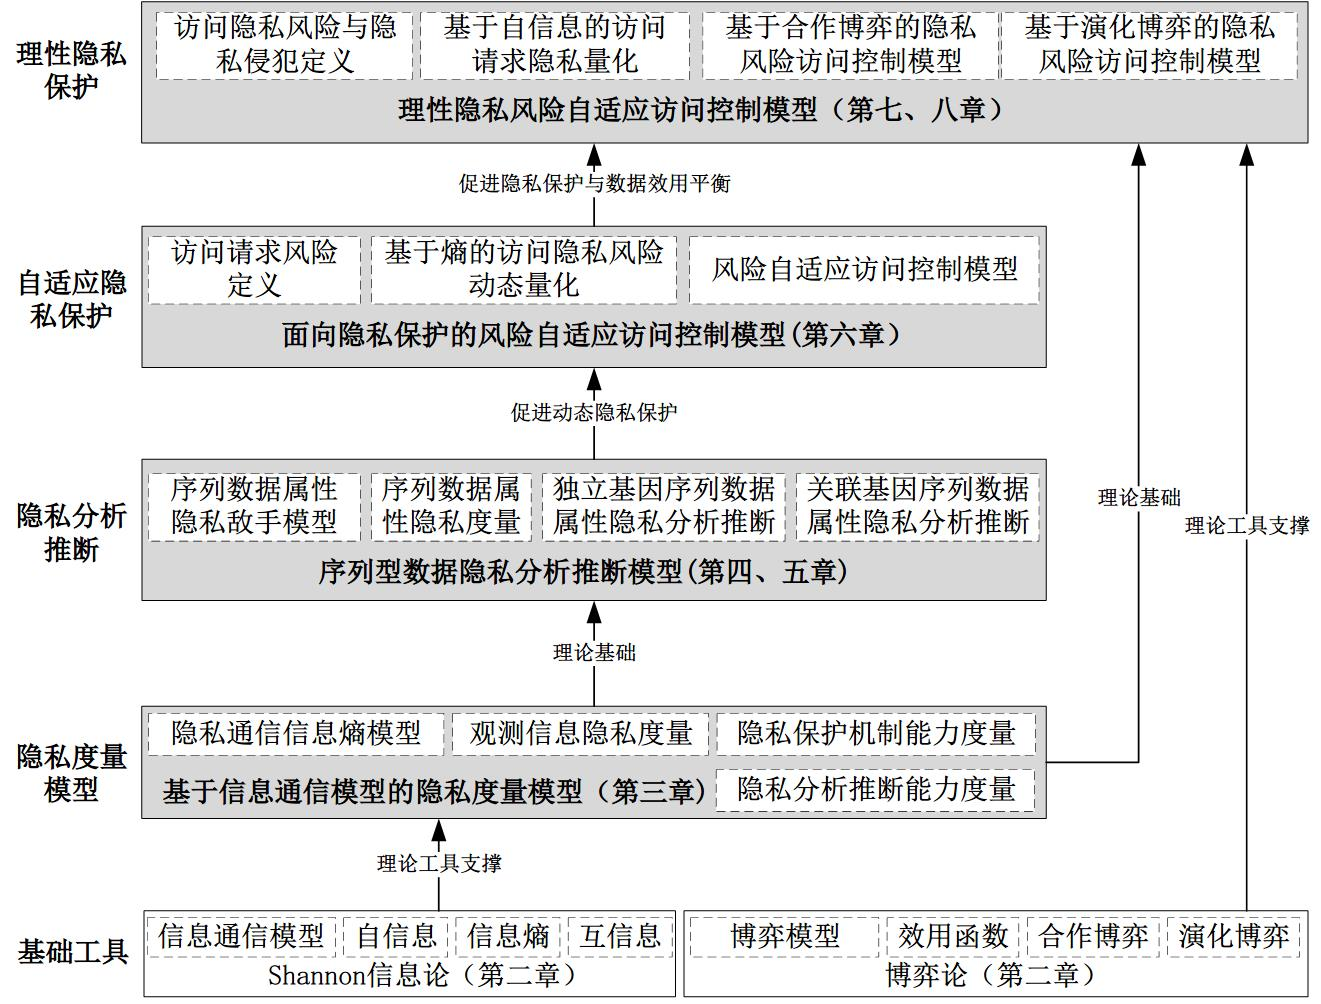
\includegraphics[width = 0.99\linewidth]{./figures/chapter1-research-framework.jpg}
	\caption{本文研究内容和框架结构}
	\label{fig:chapter1-research-framework}
\end{figure}
\subsection{基于信息熵的隐私通信模型及度量方法}
%\subsection{隐私通信模型及度量方法}
利用信息论的相关工具,如熵、互信息等来对匿名隐私、成员关系隐私和属性隐私进行形式化定义和度量的研究较多,但是大部分是集中在位置匿名、轨迹匿名、数据集匿名、数据集成员属性、训练集关系隐私、社交网络匿名和属性等方面的研究。在隐私量化方面,缺乏对隐私定义、隐私分析、隐私保护等统一的量化方法。

本文基于Shannon信息论的通信模型框架提出了几种隐私保护信息通信模型~\cite{peng2016privacy},对不含敌手的隐私保护、含敌手的隐私保护、多隐私保护源的隐私保护等不同情境提出了相应的模型进行建模,以满足对隐私度量、隐私保护机制效果度量和敌手隐私分析强度度量等需求。在所提出的度量模型中,将信息拥有者假设为发送方,隐私谋取者假设为接收方,隐私的泄露渠道假设为通信信道;基于该假设,分别引入信息熵、平均互信息量、条件熵及条件互信息等来分别描述隐私保护系统信息源的隐私度量、隐私泄露度量、含背景知识的隐私度量及泄露度量,形成了以信息论为核心的隐私度量方法体系;以此为基础,进一步提出了隐私保护方法的强度和敌手攻击强度的量化,为隐私泄露的量化提供了一种支撑,对整个隐私保护过程中的保护机制、敌手能力都提供了量化方法。%;最后,针对位置隐私保护的应用场景,通过所提出的隐私信息通信模型给出了具体的信息熵模型、以及隐私保护机制和攻击强度的度量及分析。

\subsection{独立序列型数据属性隐私推断模型}
近年来,由于数据种类繁多、数量庞大且应用需求多样化,越来越多的数据被以集中或分布式的形式共享、开放,造成了大量的隐私泄露,这些泄露又成为敌手进行隐私分析的背景知识,增加了数据共享的隐私泄露风险,对数据隐私泄露的潜在威胁量化,对数据隐私保护机制设计都提出了高的要求。特别是需要对隐私泄露的原理进行进一步研究,以帮助更好地度量隐私、理解隐私泄露机理,并设计更好的隐私保护方法。目前针对匿名方法的去匿名性分析研究较多,针对社交网络的用户偏好、个人信息等属性隐私的分析研究较多,但是对新型序列化数据的属性隐私,如时间序列的位置隐私、基因序列的基因座敏感值隐私较少,此类数据在很多共享应用场景(如疾病诊断、车联网导航)中需要非匿名化,需要对其敏感的属性隐私(特定基因座的基因型,特定行车位置)进行保护。

本文针对基因序列数据的属性隐私提出了一种基于概率推断的隐私分析模型。该模型通过对单条敏感数据记录属性值存在的相互关联关系进行分析,构建目标属性值推断的敌手模型。在提出的敌手模型基础上,分别提出了两种不同的基因序列属性隐私分析方法\cite{ding2010inferences}。第一种主要基于Monte Carlo-Markov抽样和隐Markov推断算法,建立了目标基因序列的“抽样解析”——“单倍体属性值概率推断”——“二倍体合成”三个步骤的属性隐私推断模型;第二种方法应用卷积神经网络构建概率推断算法,改进了单倍体属性值推断过程,实现了大规模序列型数据的属性推断目标。所提出的方法针对不存在亲属关系的群体基因序列数据共享场景,在本文第\ref{chap:entropy-metric-model}章提出的隐私度量模型基础上,定义了序列型数据属性隐私和量化方法,并应用于分析属性隐私泄露情况,通过量化隐私泄露量和敌手获取隐私量等信息,提高对序列型数据属性隐私的认识和理解。实验表明,本文提出的方法比现有基因序列属性隐私分析模型和算法更优,敌手对属性隐私的错误率、不确定度降低,敌手获得隐私信息量都比已有的工作更优。
\subsection{关联序列型数据属性隐私推断模型}

随着不同机构和个人更加容易获取基因组数据,且这些敏感数据被广泛地应用于医疗、保险、寻亲及社交等场景,对数据安全和隐私的担忧也在不断加剧。为了证实在序列型数据属性隐私方面,存在个人共享基因数据也会大量泄漏他人属性隐私的问题,为了进一步分析家族成员基因序列数据共享会造成他人基因序列属性隐私泄露的机理,需要对相互关联的基因序列型数据进行隐私分析。

本文利用因子图和置信传播算法针对亲属间的基因序列属性隐私建立分析推断敌手模型和分析算法。该模型考虑了单核苷酸多态性间高阶相关性,利用公开DNA参照数据集和全基因组关联研究(GWAS)目录数据,提高了推断攻击模型的属性隐私分析强度。该模型的敌手隐私分析强度通过本文所提出的隐私度量框架,对基因序列属性隐私进行了定义,并将隐私损失量作为评价指标进行了隐私分析强度量化。实验结果表明,所提出的攻击更适合于高密度基因组数据隐私推断,且具有较少的错误率、不确定性和更多隐私损失,显著提高了属性隐私的隐私分析推断能力。

\subsection{隐私保护风险自适应访问控制模型}
在以数据为中心的开放系统中,数据往往通过云服务或其他集中式的方式按需提供数据共享、开放、应用服务,这些需求多样复杂产生了复杂的隐私泄露风险和威胁,需要需要动态化、细粒度、适应性的方案对数据提供访问控制模式的隐私保护。但目前基于传统的强制访问控制、基于角色访问控制以及新型的基于属性访问控制,都不能很好的解决该问题。

本文针对云环境中共享、应用涉及隐私或敏感信息数据的场景研究面向隐私保护的访问控制模型\cite{ding2019risk}。在XACML上扩展提出了一种基于风险的自适应访问控制模型,以动态化地在访问控制过程中保护数据隐私,约束隐私侵犯行为,激励诚实访问行为。首先,根据风险访问控制场景的隐私保护需求提出了面向隐私保护的风险访问控制敌手模型;其次,该模型在标准的XACML框架进行了扩展,新增了策略风险评估、会话控制和风险消减服务三个组件,增强了策略执行、策略访问和策略信息组件。在新增的组件中,以Shannon信息熵作为工具,在第\ref{chap:entropy-metric-model}章提出的隐私度量模型基础上,提出了基于风险的隐私定义和量化方法,对用户的访问控制请求风险和用户自身的风险类型结合,提出了访问请求类型判别方法;通过风险隐私量化及基于信用卡模型的激励机制,实现访问行为风险阈值的动态调整,考虑了用户短期访问行为和长期访问行为的影响。对比和分析表明,所提出的模型和方法较现有的工作更加动态化,且实现了隐私保护,易用性更好。
\subsection{基于扩展式博弈的理性隐私风险访问控制模型}

基于风险访问控制模型可很好的解决以数据为中心的开放系统中自适应数据隐私保护。但强制访问控制、基于角色访问控制、基于属性访问控制和已有的基于风险访问控制等模型,在平衡隐私保护需求与数据效用需求冲突方面,仍存在问题,特别是过度授权导致隐私泄露或授权不足导致数据可用性不足的问题需要进一步解决。此外,还需要对基于风险访问模型中对隐私保护的能力和方法进一步提升。

针对上述需求和问题,本文在所提出的风险自适应访问控制模型的基础上,进一步运用Shannon自信息和博弈论,提出了基于风险适应性的理性访问控制模型以实现数据共享场景中的保护隐私和数据应用需求间的平衡\cite{ding2019game}。在定义了隐私风险和隐私侵犯访问的概念之后,提出了基于博弈论的风险访问控制模型框架和工作流程。此外,还进一步利用Shannon信息的定义提出了量化访问请求隐私风险和用户隐私风险值的计算公式,强化了访问控制请求对数据隐私的刻画;以提出的理性风险访问控制模型、访问请求隐私 风险和用户隐私风险为基础,提出了多轮二人博弈来刻画面向隐私保护的风险访问控制中访问者与数据服务提供者的“隐私保护-数据服务”冲突与合作关系,进一步提出并分析了博弈效用函数及其二人博弈过程。分析表明,在基于隐私风险访问控制的每一轮博弈中都存在子博弈精炼纳什均衡,可以通过限制侵犯隐私的访问请求来保护隐私,实现隐私保护与数据访问效用间的平衡。分析和对比表明,该方法比已有的工作更有优势,需要更少的辅助信息,提供更多的风险适应性和隐私保护强度。

\subsection{基于演化博弈的理性隐私风险访问控制模型}

社交网络、医疗信息系统等以数据为中心的大规模用户(访问者)开放信息系统,亟需能够保护隐私的细粒度自适应访问控制模型,且需实现数据隐私保护需求和数据效用需求的平衡。现有基于理性的访问控制模型难以满足适应性保护隐私的需求,且博弈参与者的完全理性假设太强,不符合实际场景。基于风险访问控制能够实现细粒度的访问控制隐私保护目标,但如何进一步放松参与者完全理性的假设,并实现隐私保护与数据效用关系的动态平衡,仍需要进一步研究。

本文针对这些问题和需求,在提出的风险自适应访问控制模型和完全理性隐私风险访问控制模型的基础上,进一步提出一种面向隐私保护的有限理性风险自适应访问控制模型。新提出的模型包含了新的隐私风险量化模块和演化博隐私弈决策模块。该模型首先基于信息量对访问请求的数据集隐私信息量进行量化,构造了访问请求隐私风险函数和用户隐私风险函数;其次,基于演化博弈在有限理性假设下构建多参与者的访问控制演化博弈模型,利用复制动态方程分析了访问控制参与者的动态策略选择和演化稳定状态形成机理,提出了隐私风险访问控制博弈演化稳定策略的选取方法。仿真实验和对比表明,所提出的访问控制模型能够有效动态自适应地保护敏感信息资源系统中的隐私信息,具有更好的隐私风险适应性,有限理性参与者的动态演化访问策略选取更加符合实际场景。

\section{论文结构安排}

本文其余部分的结构如图~\ref{fig:chapter1-research-framework}所示,具体安排如下:第~\ref{chap:preliminary}章介绍本文研究所涉及的信息论、博弈论及隐私保护等共性基本概念,包括Shannon信息论,策略博弈、扩展博弈等博弈论概念,隐私分类及隐私保护基本模型;接下来,分为四部分论述本文的主要工作。首先利用信息论作为基础工具,为隐私度量提出了一个基于通信模型的统一框架模型,提出了隐私定义与量化、隐私分析强度量化和隐私保护机制能力量化的模型与基本方法(详见第\ref{chap:entropy-metric-model}章);其次,针对以数据共享应用为场景,以基于信息论的序列属性隐私定义和量化为基础,面向序列型数据的属性隐私建立了属性值推断分析敌手模型和概率推断分析方法,对相互独立基因序列数据隐私和具备树状图结构关联的基因序列数据隐私进行了隐私分析推断(详见第\ref{chap:inference-attack-on-norelated-sequenced-data}与第\ref{chap:inference-attack-on-related-sequenced-data}章);再次,以访问请求和用户风险定义和量化为基础,针对数据共享应用场景中的细粒度数据隐私保护需求,设计并提出了一种面向隐私保护的风险自适应访问控制模型(详见第\ref{chap:RaBAC-for-privacy}章);最后,在进一步强化用户访问请求的隐私侵犯刻画的基础上,提出了基于博弈论的理性风险访问控制,分别对完全理性参与者和有限理性参与者的隐私保护访问控制进行建模和分析,以平衡隐私保护与数据效用间关系的平衡(详见第\ref{chap:game-theoretical-RaBAC-for-privacy}和第\ref{chap:evolutionary-rabac}章)。
